\documentclass[compress,red]{beamer}
\usepackage[utf8]{inputenc}
\usepackage{ucs}
\usepackage{amsmath}
\usepackage{amsfonts}
\usepackage{amssymb}
\usepackage[russian]{babel}
\usepackage{graphicx}
\usepackage{wrapfig}

\usepackage{tikz}
\usepackage{verbatim}

\usepackage{color}
\usepackage{xcolor}
\usepackage{listings}

\usepackage{caption}

\lstset{
language=ruby,
extendedchars=\true,
inputencoding=utf8x,
commentstyle=\itshape,
stringstyle=\bf,
belowcaptionskip=5pt }

\DeclareCaptionFont{white}{\color{white}}
\DeclareCaptionFormat{listing}{\colorbox{gray}{\parbox{\textwidth}{#1#2#3}}}
\captionsetup[lstlisting]{format=listing,labelfont=white,textfont=white}

\usetikzlibrary{calc,trees,positioning,arrows,chains,shapes.geometric,%
    decorations.pathreplacing,decorations.pathmorphing,shapes,%
    matrix,shapes.symbols}

\tikzset{
>=stealth',
  punktchain/.style={
    rectangle, 
    rounded corners, 
    % fill=black!10,
    draw=black, very thick,
    text width=10em, 
    minimum height=3em, 
    text centered, 
    on chain},
  line/.style={draw, thick, <-},
  element/.style={
    tape,
    top color=white,
    bottom color=blue!50!black!60!,
    minimum width=8em,
    draw=blue!40!black!90, very thick,
    text width=10em, 
    minimum height=1.5em, 
    text centered, 
    on chain},
  every join/.style={->, thick,shorten <=1pt},
  decoration={brace},
  tuborg/.style={decorate},
  tubnode/.style={midway, right=2pt},
}

\mode<presentation>

\usetheme{Warsaw}

\definecolor{Red}{rgb}{1,0,0}
\definecolor{Blue}{rgb}{0,0,1}
\definecolor{Green}{rgb}{0,1,0}
\definecolor{magenta}{rgb}{1,0,.6}
\definecolor{lightblue}{rgb}{0,.5,1}
\definecolor{lightpurple}{rgb}{.6,.4,1}
\definecolor{gold}{rgb}{.6,.5,0}
\definecolor{orange}{rgb}{1,0.4,0}
\definecolor{hotpink}{rgb}{1,0,0.5}
\definecolor{newcolor2}{rgb}{.5,.3,.5}
\definecolor{newcolor}{rgb}{0,.3,1}
\definecolor{newcolor3}{rgb}{1,0,.35}
\definecolor{darkgreen1}{rgb}{0, .35, 0}
\definecolor{darkgreen}{rgb}{0, .6, 0}
\definecolor{darkred}{rgb}{.75,0,0}

\xdefinecolor{olive}{cmyk}{0.64,0,0.95,0.4}
\xdefinecolor{purpleish}{cmyk}{0.75,0.75,0,0}

\useoutertheme[subsection=false]{smoothbars}

\title{Алгоритмы. Перебор и рекурсия.}
\author{Информатика \\ 10-11 классы}

%\usecolortheme{dolphin}


\begin{document}
%%титульная страница
\maketitle
%% основные моменты

\section{Алгоритмы}
\subsection{Алгоритмы}
\begin{frame}[fragile]
\frametitle{Что такое алгоритм?}
		\begin{itemize}
		\item Алгоритм — это конечный набор правил, который определяет последовательность операций для решения конкретного множества задач и обладает пятью важными чертами: конечность, определённость, ввод, вывод, эффективность (Д. Кнут).
		\item Основные свойства алгоритма:
		  \begin{enumerate}
		    \item Дискретность --- последовательное выполнение простых шагов.
		    \item Детерменированность  --- определённость --- одинаковые исходные данные дают одинаковый результат.
		    \item Понятность.
		    \item Конечность --- количество шагов должно быть конечно (может быть и неявно задано).
		    \item Универсальность --- алгоритм должен работать для множества исходных данных.
		  \end{enumerate}
		\end{itemize}
\end{frame}

\subsection{Алгоритмы}
\begin{frame}[fragile]
\frametitle{Виды алгоритмов}
  \begin{enumerate}
    \item Динамическое программирование (было).
    \item Метод перебора.
    \item Рекурсия (повторение через себя). \emph{Рекурсия --- это рекурсия}.
    \item Жадные алгоритмы (хватай сначала самое большое).
    \item Разделяй и властвуй (привет, принцип 3 ветвей власти).
    \item Метод двоичного поиска.
    \item Много--много других.
  \end{enumerate}
\end{frame}

\section{Перебор}
\subsection{Метод перебора}
\begin{frame}[fragile]
  \frametitle{Метод перебора}
	\begin{itemize}
	  \item Идея метода перебора очень проста --- переберём все варианты и выберем только те, которые нам нужны.
	  \item Рассмотрим простую задачу: вывести на экран простые числа <= N.
	  \item Есть красивые решения типа решета Эратосфена. Но мы пойдём ``в лоб''.
  \end{itemize}
  \scriptsize{
  \begin{lstlisting}[label=ruby1,caption=Простые числа]
    def is_prime?(n)
      return false if ((n == 1) || (n == 0))
      for i in 2..(n-1)
        return false if (n%i == 0)
      end
      true
    end
    
    100.times {|i| puts i if is_prime?(i) }
  \end{lstlisting}}}
  
\end{frame}

\subsection{Посложнее}
\begin{frame}[fragile]
  \frametitle{Метод перебора: НОД}
	\begin{itemize}
	  \item Рассмотрим задачу: найти НОД($a$,$b$).
	  \item Пример: НОД(15,12) = 3
	  \item Решаем методом перебора.
	  \item Переберём все возможные делители этих двух чисел.
	  \item Для этого пройдёмся циклом от 2 до, например, $a$.
	  \item Если оба числа делятся на пробегаемое число, значит, пробегаемое число --- делитель. Запоминаем его.
	  \item Если в результате работы программы мы находим делитель, который больше запомненного ранее, то стираем старый и записываем новый.
	  \item Изначально зададим НОД = 1 (на 1 все числа делятся).
	  \item НОД по-английски --- gcd.
  \end{itemize}
\end{frame}

\subsection{Посложнее}
\begin{frame}[fragile]
  \frametitle{Метод перебора: НОД}
  \begin{lstlisting}[label=ruby2,caption=НОД(a,b)]
    def gcd(a,b)
      max = 1
      for i in 2..a
        max = i if ((a%i==0) && (b%i==0))
      end
      max
    end

    a = 126
    b = 486
    
    puts gcd(a,b)
  \end{lstlisting}}
  
\end{frame}

\subsection{Задачи}
\begin{frame}[fragile]
  \frametitle{Задачи на метод перебора}
	\begin{itemize}
	  \item Задача 1. Дано некоторое число $a$. Вывести на экран все числа, которые взаимно просты с $a$ и не превышают $N$. $N$ задаётся также в начале программы.
	  \item Пример: a = 3, N = 10. Программа должна вывести следующие числа: 2, 4, 5, 7, 8, 10.
	  \item Задача 2. Вывести на экран все пары взаимно простых чисел, каждое из которых не превышает $N$. $N$ задаётся в начале программы.
	  \item Пример: N = 5. Программа должна вывести: (2,3), (2,5), (3,4), (3,5), (4,5).
  \end{itemize}
\end{frame}

\section{Рекурсия}
\subsection{Рекурсия1}
\begin{frame}[fragile]
\frametitle{Рекурсия}
  \begin{figure}
    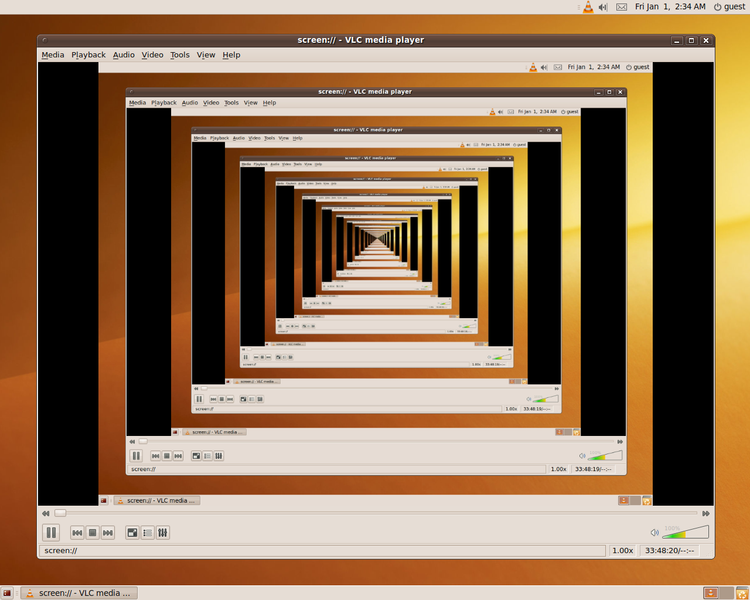
\includegraphics[width=0.7\textwidth]{images/recursion1.png}
    \caption{\scriptsize{Источник: http://ru.wikipedia.org}}}
  \end{figure}
\end{frame}

\subsection{Рекурсия2}
\begin{frame}[fragile]
\frametitle{Рекурсия}
  \begin{figure}
    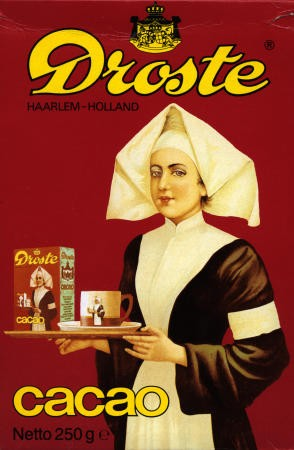
\includegraphics[width=0.4\textwidth]{images/recursion2.jpg}
    \caption{\scriptsize{Источник: http://ru.wikipedia.org}}}
  \end{figure}
\end{frame}

\subsection{Рекурсия}
\begin{frame}[fragile]
\frametitle{Рекурсия}
		\begin{itemize}
		\item Рекурсия --- это рекурсия.
		\item Рекурсия --- это когда функция использует сама себя.
		\item Пример рекурсии --- числа Фибоначчи. Для того, чтобы посчитать 10 число Фибоначчи, нужно знать 8 и 9. А чтобы узнать их, нужно знать 2 их предыдущих и так далее.
		\item У рекурсии всегда есть две составляющие:
		  \begin{enumerate}
		    \item База --- до какого момента спускаемся. В случае чисел Фибоначчи база --- это нулевое и первое числа, которые равны 1.
		    \item Рекуррентная формула --- формула, которая говорит, как получить что-то из предыдущего. Для чисел Фибоначчи это: число Фибоначчи равно сумме двух предыдущих ($\varphi_n = \varphi_{n-1} + \varphi_{n-2}$)
		  \end{enumerate}
		\item Рекурсия может быть медленной.
		\end{itemize}
\end{frame}

\subsection{Числа Фибоначчи: рекурсия}
\begin{frame}[fragile]
  \frametitle{Числа Фибоначчи: рекурсия}
	\begin{itemize}
	  \item Напишем функцию для вычисления n--ного числа Фибоначчи через рекурсию.
	  \item (!) Сравните по времени, сколько вычисляется 50-е число Фибоначчи рекурсией и обычным циклом.
  \end{itemize}
  \scriptsize{
  \begin{lstlisting}[label=ruby3,caption=Рекурсия для чисел Фибоначчи]
    def fibonacci(n)
      return 1 if ((n==0) || (n==1))
      fibonacci(n-1)+fibonacci(n-2)
    end
    
    puts fibonacci(10)
  \end{lstlisting}}}
  
\end{frame}

\subsection{Легенда о Ханойских башнях}
\begin{frame}[fragile]
\frametitle{Легенда о Ханойских башнях}
  \begin{itemize}
  \item Легенда гласит, что в Великом храме города Бенарас, под собором, отмечающим середину мира, находится бронзовый диск, на котором укреплены 3 алмазных стержня, высотой в один локоть и толщиной с пчелу. Давным-давно, в самом начале времён, монахи этого монастыря провинились перед богом Брахмой. Разгневанный, Брахма воздвиг три высоких стержня и на один из них возложил 64 диска. Брахма поместил на один из стержней 64 диска из чистого золота, причем так, что каждый меньший диск лежит на большем.
  \item Как только все 64 диска будут переложены со стержня, на который Брахма сложил их при создании мира, на другой стержень, башня вместе с храмом обратятся в пыль и под громовые раскаты погибнет мир.
  \end{itemize}
\end{frame}

\subsection{Задача о ханойских башнях}
\begin{frame}[fragile]
\frametitle{Задача о ханойских башнях}
  \begin{figure}
    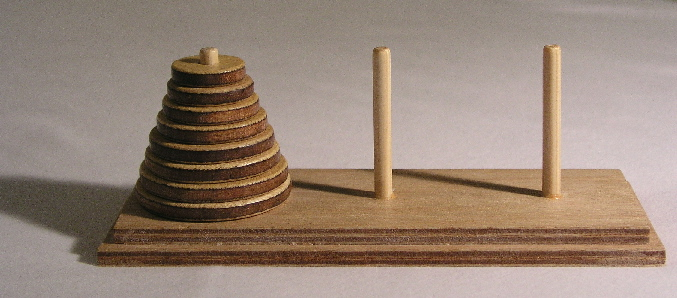
\includegraphics[width=0.8\textwidth]{images/hanoi.jpeg}
    \caption{\scriptsize{Источник: http://ru.wikipedia.org}}}
  \end{figure}
\end{frame}

\subsection{Ханой}
\begin{frame}[fragile]
\frametitle{Задача о ханойских башнях}
		\begin{itemize}
		\item Пример простого решения рекурсией \textbf{без понимания} работы алгоритма --- задача о ханойских башнях.
		\item Даны три стержня, на один из которых нанизаны несколько колец, причем кольца отличаются размером и лежат меньшее на большем. Задача состоит в том, чтобы перенести пирамиду из восьми колец за наименьшее число ходов. За один раз разрешается переносить только одно кольцо, причём нельзя класть большее кольцо на меньшее.
		\item Пример алгоритма для 3 колец: с 1 на 3, с 1 на 2, с 3 на 2, с 1 на 3, с 2 на 1, с 2 на 3, с 1 на 3.
		\item \scriptsize{Задача 1. Написать программу с использованием рекурсии, которая выводит на экран алгоритм решения задачи для заданного количества колец.}
		\item \scriptsize{Задача 2. Посчитать и объяснить, сколько минимально потребуется монахам времени, чтобы выполнить условие Брахмы. Предположим, что на 1 перекладывание монахи тратят 1 минуту.}
		\end{itemize}
\end{frame}

\section{References}
\subsection{References}
\begin{frame}[fragile]
  \frametitle{References}
  \begin{itemize}
    \item Все презентации доступны на http://school.smirik.ru!
    \item Вопросы, предложения, д/з: smirik@gmail.com
  \end{itemize}
\end{frame}

\end{document}
